\documentclass[12pt,a4paper]{article}

% ---------- Кодирање и језик (XeLaTeX) ----------
\usepackage{fontspec}
\usepackage{polyglossia}
\setdefaultlanguage{serbian}
\setmainfont{DejaVu Serif}

% ---------- Пакети ----------
\usepackage{graphicx}
\usepackage{amsmath, amssymb}
\usepackage{amsthm}
\usepackage{xcolor}
\usepackage{wrapfig}
\usepackage{booktabs}
\usepackage{geometry}
\usepackage{enumitem}
\usepackage[colorlinks=true, linkcolor=svemirplava, urlcolor=svemirplava, citecolor=svemirplava]{hyperref}

\geometry{margin=2.5cm}

% ---------- Боје ----------
\definecolor{svemirljubicasta}{HTML}{6A4FD6}
\definecolor{svemirplava}{HTML}{1E6FBF}
\definecolor{svemirzlatna}{HTML}{C97A1A}

% ---------- Дефиниције, теореме, леме ----------
\newtheorem{teorema}{Теорема}
\newtheorem{definicija}{Дефиниција}
\newtheorem{lema}{Лема}

\title{\textbf{\textcolor{svemirljubicasta}{Сунчев систем и основни закони небеске механике}}}
\author{Ана Ћалић \\ \small Број индекса: МИ25192}
\date{\today}

\begin{document}

\maketitle
\tableofcontents
\newpage

\section{Увод}

Од најстаријих цивилизација до данас, човек посматра небо покушавајући
да разуме законитости које управљају кретањем небеских тела. Овај рад
даје сажет преглед настанка \textbf{Сунчевог система}, поделе планета и
основних закона небеске механике који описују њихово кретање, уз
неколико занимљивости о свакој планети понаособ.

\subsection{Мотивација}

Циљ рада је да на \textbf{сажет}, али \textit{информативан} начин
прикаже кључне чињенице о Сунчевом систему, уз
\textcolor{svemirplava}{математички} опис кретања планета и кратак
осврт на његов настанак.

\section{Настанак Сунчевог система}

Сунчев систем је настао пре отприлике \textcolor{svemirzlatna}{4,6
милијарди година}, колапсом огромног облака гаса и прашине познатог
као \textbf{соларна маглина}. Под дејством сопствене гравитације,
највећи део материјала се сажео у центру и формирао \textbf{Сунце},
док је преостали диск гаса и прашине постепено формирао планете,
месеце, астероиде и комете.

\begin{wrapfigure}{l}{0.36\textwidth}
  \centering
  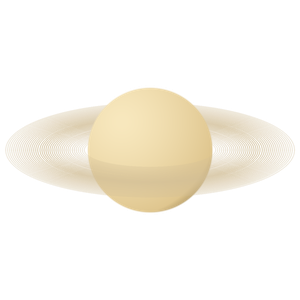
\includegraphics[width=0.34\textwidth]{slike/saturn.png}
  \caption{Сатурн са препознатљивим системом прстенова}
\end{wrapfigure}

Планете ближе Сунцу изгубиле су већи део лаких гасова услед сунчевог
зрачења, па су остале \textit{стеновите}, док су планете у спољашњем,
хладнијем делу система задржале дебеле атмосфере водоника и хелијума,
постајући \textit{гасовити дивови}. Управо тај распоред -- мали и
густи светови близу Сунца, велики и лаки светови далеко од њега --
једна је од најупечатљивијих карактеристика нашег система.

\subsection{Подела планета}

Планете Сунчевог система деле се у две основне групе, према саставу и
физичким особинама.

\section{Закони кретања планета}

Почетком 17. века, Јохан Кеплер је, анализирајући астрономска
посматрања Тиха Браеа, формулисао три закона који описују кретање
планета око Сунца.

\begin{definicija}
\textbf{Елипса} је геометријско место тачака за које је збир
растојања до две фиксиране тачке (жиже) константан. По елиптичним
путањама крећу се све планете Сунчевог система.
\end{definicija}

\begin{teorema}[Кеплеров трећи закон]
Квадрат периода револуције планете сразмеран је кубу њене средње
удаљености од Сунца:
\[
T^2 \propto a^3
\]
где је $T$ период револуције, а $a$ средње растојање планете од Сунца.
\end{teorema}

\begin{lema}
Из Кеплеровог другог закона следи да се планета креће брже када је
ближа Сунцу (у перихелу), а спорије када је даље од њега (у афелу),
будући да дуж која спаја планету и Сунце у једнаким временским
интервалима преброди једнаке површине.
\end{lema}

Њутн је касније показао да Кеплерови закони директно следе из општег
закона гравитације:
\[
F = G \frac{m_1 m_2}{r^2}
\]
где је $F$ гравитациона сила између два тела маса $m_1$ и $m_2$, $r$
растојање међу њима, а $G$ гравитациона константа. Овај закон важи не
само за планете, већ и за све остале интеракције у васиони -- баш као
што позната Ајнштајнова релација
\[
E = mc^2
\]
описује еквиваленцију масе и енергије, тако Њутнов закон описује
универзалну природу гравитације.

\section{Преглед планета}

Табела~\ref{tab:planete} приказује основне податке о свих осам
планета Сунчевог система, поређаних по удаљености од Сунца.

\begin{table}[h]
\centering
\caption{Основни подаци о планетама Сунчевог система}
\label{tab:planete}
\begin{tabular}{lp{2.6cm}p{2.6cm}p{2.6cm}}
\toprule
\textbf{Планета} & \textbf{Тип} & \textbf{Пречник (km)} & \textbf{Растојање (АЈ)} \\
\midrule
Меркур  & Стеновита     & 4\,879   & 0,39 \\
Венера  & Стеновита     & 12\,104  & 0,72 \\
Земља   & Стеновита     & 12\,742  & 1,00 \\
Марс    & Стеновита     & 6\,779   & 1,52 \\
Јупитер & Гасовити див  & 139\,820 & 5,20 \\
Сатурн  & Гасовити див  & 116\,460 & 9,58 \\
Уран    & Ледени див    & 50\,724  & 19,22 \\
Нептун  & Ледени див    & 49\,244  & 30,05 \\
\bottomrule
\end{tabular}
\end{table}

\section{Занимљивости и подела}

Подела планета према саставу може се представити на више начина:

\begin{enumerate}[label=\arabic*)]
  \item \textbf{Терестријалне (стеновите) планете} -- Меркур, Венера, Земља и Марс;
  \item \textbf{Гасовити дивови} -- Јупитер и Сатурн;
  \item \textbf{Ледени дивови} -- Уран и Нептун.
\end{enumerate}

Поред основне поделе, издвајамо и неколико занимљивих чињеница:

\begin{itemize}[label=--]
  \item Један дан на Венери траје дуже од њене године;
  \item Јупитерова Велика црвена пега бесни већ најмање неколико векова;
  \item Сатурнови прстенови дебели су свега неколико десетина метара;
  \item Нептун је откривен математичким предвиђањем, пре непосредног посматрања.
\end{itemize}

Хронолошки редослед открића спољашњих планета може се представити и као:

\begin{description}
  \item[1781.] откриће Урана (Вилијам Хершел);
  \item[1846.] откриће Нептуна (на основу прорачуна Ле Веријеа);
  \item[1930.] откриће патуљасте планете Плутон (касније искључене из главне поделе).
\end{description}

\section{Закључак}

Сунчев систем представља складан резултат гравитационог обликовања
облака гаса и прашине пре милијарди година. Кеплерови закони, а
касније и Њутнов закон гравитације, омогућили су прецизно
математичко описивање кретања планета, чиме је небеска механика
постала једна од најегзактнијих грана физике. Разумевање ових
основних принципа и данас представља темељ за проучавање не само
нашег система, већ и бројних егзопланетарних система откривених
ван њега.

\end{document}
